% !TeX root = ../../thesis.tex
% ------------------------------------------------
\StartChapter{System Design}{chapter:system-design}
% ------------------------------------------------

Google \RefBib{website:google}

Papaer \RefBib{diego2019iotsafe}

Figure \RefTo{fig:docker_architecture}

Table \RefTo{table:table_1}

\InsertFigure
  [scale=0.9, caption={Docker Architecture \unexpanded\expandafter{\RefBib{book:docker-build}}}, label={fig:docker_architecture}]
  {./context/figures/docker_architecture.png}

\clearpage

\begin{table}[h!]
  \caption{Redis}
  \label{table:table_1}
  \setlength{\tabcolsep}{6pt}
  \renewcommand{\arraystretch}{1.6}
  \centering
  \resizebox{\linewidth}{!}
  {
    \scalebox{0.02}
    {
      \begin{tabular}{|c|c|c|c|c|}
      \hline
      \diagbox{X}{Y}
      & A & B & C & D \\ \hline
      1 & \checkmark & \checkmark & \checkmark  & \checkmark \\ \hline
      2 & \checkmark & \checkmark & \checkmark  & \\ \hline
      3 & \checkmark &            &             & \\ \hline
      4 &            &            &             & \\ \hline
      \end{tabular}
    }
  }
\end{table}

\bigbreak

\begin{table}[h!]
  \caption{Environment}
  \label{table:table_2}
  \setlength{\tabcolsep}{6pt}
  \renewcommand{\arraystretch}{1.6}
  \begin{adjustbox}{width=1.1\textwidth,center}
    \begin{tabular}{|l|l|l|l|l|}
      \hline
      & Nvidia Jetson TX2 & Raspberry Pi 3 Model B & VM0 (ESXi 6.0) & VM1 (ESXi 5.5) \\ \hline
      CPU & 2 x 2 GHz + 4 x 2 GHz & 4 x 1.2 GHz & 8 x 3.70 GHz & 8 x 3.40 GHz \\ \hline
      GPU & Nvidia Pascal 256-core & Broadcom VideoCore & None & None \\ \hline
      RAM & 8GB & 1 GB & 12 GB & 2 GB \\ \hline
      Ethernet & 1 Gb/s & 100 Mb/s & 1 Gb/s & 1 Gb/s \\ \hline
      OS & Ubuntu 16.04.6 LTS & Raspbian 9.9 (stretch) & Xubuntu 16.04.6 LTS & Ubuntu Server 18.04.2 LTS \\ \hline
      Linux kernel & TX2 4.4.38-tegra \textbf{aarch64} & RPi 4.19.50-v7+ \textbf{armv7l} & 4.15.0-52-generic \textbf{x86\_64} & 4.15.0-45-generic \textbf{x86\_64} \\ \hline
      Software package & Docker 18.09.7 & Docker 18.09.0 & Docker 18.09.6 & Docker 18.09.6 \\ \hline
    \end{tabular}
  \end{adjustbox}
\end{table}

\clearpage

\begin{table}[h!]
  \caption{Timetable}
  \label{table:table_3}
  \centering
  \begin{tabular}{|c|c|c|c|}
    \hline
    \diagbox{X}{Y}
          & A & B & C \\ \hline
    22:03 & 1       & 1      & 1    \\ \hline
    22:12 & 1       & 10     & 10   \\ \hline
    22:24 & 1       & 20     & 20   \\ \hline
    22:36 & 1       & 40     & 40   \\ \hline
  \end{tabular}
\end{table}

\bigbreak

\begin{figure}[h!]
  \makebox[\linewidth][c]{%
    \begin{subfigure}[b]{.4\textwidth}
      \centering
      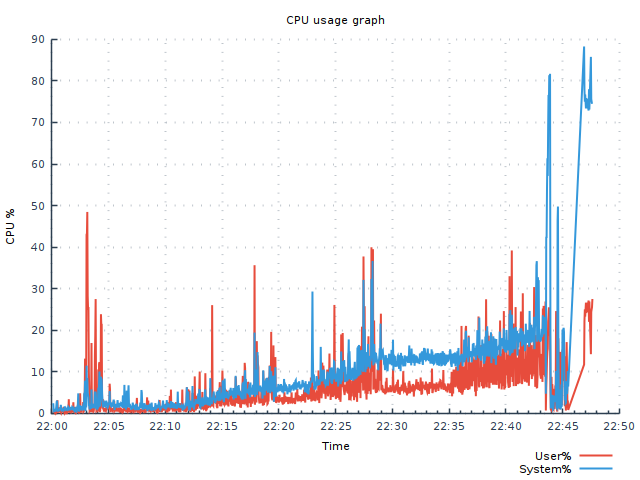
\includegraphics[width=0.95\linewidth]{./context/figures/rpi_cpu.png}
      \caption{CPU usage}
      \label{fig:rpi_cpu}
    \end{subfigure}%
    \begin{subfigure}[b]{.4\textwidth}
      \centering
      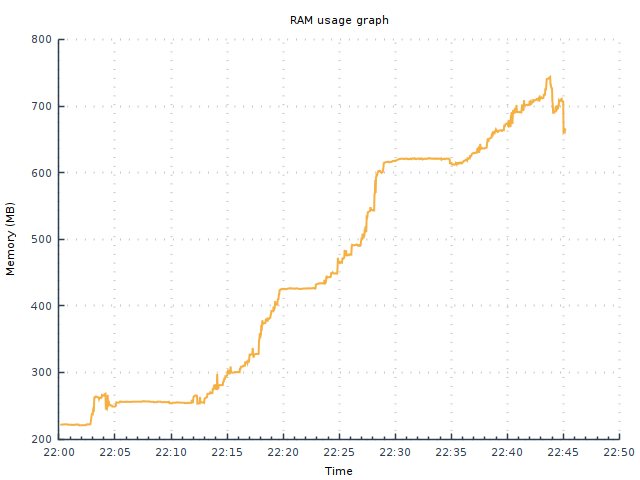
\includegraphics[width=0.95\linewidth]{./context/figures/rpi_ram.png}
      \caption{RAM usage}
      \label{fig:rpi_ram}
    \end{subfigure}
    \centering
    \begin{subfigure}[b]{.4\textwidth}
      \centering
      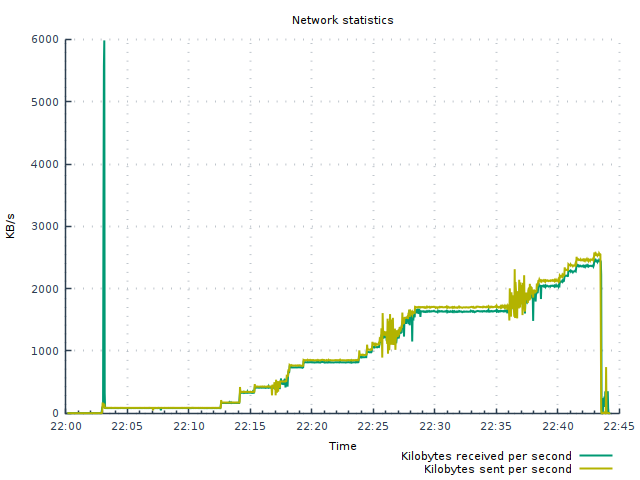
\includegraphics[width=0.95\linewidth]{./context/figures/rpi_netinterface.png}
      \caption{Network throughput}
      \label{fig:rpi_netinterface}
    \end{subfigure}%
  }
  \caption{Performance}
  \label{fig:result_rpi}
\end{figure}

% ------------------------------------------------
\EndChapter
% ------------------------------------------------
